\chapter{The macro language, and your first simulation}
\label{ch:macro}

\begin{willdo}
\begin{itemize}
  \item Recognise the three families of commands a \musrSim\ macro is built from.
  \item Understand the two ways \musrSim\ reads your macro --- the key to every ``why was my line ignored?''.
  \item List the commands your executable understands.
  \item Write, run and inspect a complete simulation from a blank file.
\end{itemize}
\end{willdo}

A \musrSim\ macro (also called the \emph{steering file}) is a plain-text script. There is no compilation step: change a number, run again. Master this one file and you can build almost any instrument without touching C++.

\section{Three families of commands}
Every line in a working macro belongs to one of three families. Telling them apart is the single most useful orientation skill in this toolkit.

{\tablestyle
\begin{tabularx}{\textwidth}{@{}>{\raggedright\arraybackslash}p{0.22\textwidth} >{\raggedright\arraybackslash}p{0.27\textwidth} L@{}}
\toprule
\textbf{Family} & \textbf{Prefix} & \textbf{What it controls}\\
\midrule
Standard Geant4 & \code{/run}, \code{/vis}, \code{/tracking}, \code{/control}, \code{/process}, \code{/gps} & Universal Geant4 kernel commands, identical in every Geant4 application.\\
\musrSim\ core & \code{/musr/command} & Geometry, fields, physics processes, output selection. Read directly from the file by \musrSim's C++ (next section).\\
\musrSim\ run control & \code{/musr/run} & Random seeding, progress printout.\\
Beam (particle gun) & \code{/gun} & The muon beam model: vertex, momentum, spin, decay timing, TURTLE input, and the cosmic-ray generators.\\
\bottomrule
\end{tabularx}}

\begin{keypoint}
The \code{/run}, \code{/vis} and \code{/control} commands are documented in the official Geant4 guides and never change. The \code{/musr/...} and \code{/gun/...} commands are the ones this book teaches, because they live in your copy of the source and differ between forks. When in doubt about a \musrSim-specific command, the source is the specification.
\end{keypoint}

\section{How \musrSim\ reads a macro: twice}
\label{sec:tworeads}
This is the one piece of plumbing worth understanding before you write a line. Your macro is read in two different ways.

\begin{center}
\begin{tikzpicture}[node distance=4mm and 8mm]
  \node[box,minimum width=30mm] (file) {\textbf{your macro}\\\texttt{first\_sim.mac}};
  \node[hot,right=14mm of file,yshift=9mm,minimum width=62mm,align=left,text width=58mm] (r1) {\textbf{Read 1 --- at start-up} (\texttt{Initialize()})\\C++ scans the file for \texttt{/musr/command} lines: geometry, fields, processes, output switches.};
  \node[box,right=14mm of file,yshift=-9mm,minimum width=62mm,align=left,text width=58mm] (r2) {\textbf{Read 2 --- execution} (\texttt{/control/execute})\\Geant4 runs every line in order: \texttt{/gun}, \texttt{/musr/run}, \texttt{/vis}, \dots, \texttt{/run/beamOn}. \texttt{/musr/command} lines are skipped.};
  \draw[arr] (file.east) -- ++(5mm,0) |- (r1.west);
  \draw[arr] (file.east) -- ++(5mm,0) |- (r2.west);
\end{tikzpicture}
\end{center}

\textbf{Read 1 --- start-up.} \code{main()} first creates the detector and the physics list and calls Geant4's \code{Initialize()}. During that call \code{musrDetectorConstruction} and \code{musrPhysicsList} each open your macro \emph{as a text file} and parse every line that starts with \code{/musr/command}, top to bottom: volumes, rotations, fields, \code{rootOutput} switches, \code{process} lines.

\textbf{Read 2 --- execution.} Only then does \code{main()} run \code{/control/execute <yourfile>}. Now Geant4 executes the macro line by line as ordinary UI commands: \code{/gun/...} sets the beam, \code{/musr/run/...} sets seeding, \code{/vis/...} sets up pictures, and \code{/run/beamOn} starts the events. The \code{/musr/command} lines are passed to a messenger that deliberately ignores them --- they have already done their job.

Three practical rules follow.
\begin{enumerate}
  \item \textbf{No \code{/run/initialize}.} Initialisation has already happened before Read~2 begins; your macro simply ends with \code{/run/beamOn}.
  \item \textbf{Order matters among \code{/musr/command} lines}: a mother volume before its daughters, a rotation matrix before the volume that uses it, a volume before the field attached to it. Where they sit relative to \code{/gun} lines does not matter.
  \item \textbf{\code{/musr/command} lines must be in the macro you pass on the command line.} Read~1 does not follow \code{/control/execute}, so geometry or physics in an included file is silently never built. Included files are fine for \code{/vis} and \code{/gun} commands --- that is exactly how \code{visVRML.mac} works.
\end{enumerate}

\begin{hood}
You can see both reads in \code{musrSim.cc}: \code{runManager->Initialize()} comes first, then \code{UI->ApplyCommand("/control/execute " + fileName)}. The parsing loops are \code{musrDetectorConstruction::Construct()} and \code{musrPhysicsList::ConstructEM()}; both skip lines whose first character is \code{#}.
\end{hood}

\section{List the real commands}
\label{sec:listcommands}
Before trusting any command in any manual --- including this one --- ask your executable what it supports. Run any macro with \code{idle} as the second argument: once the macro has finished you get Geant4's \code{Idle>} prompt, where you can browse the live command tree.

\begin{lstlisting}[style=sh,caption={Discovering \texttt{/gun} and \texttt{/musr/run} commands without reading C++}]
cd build/run
../musrSim first_sim.mac idle
# at the Idle> prompt:
#   ls /gun/                       list every beam command (and /gun/cry/, /gun/ecomug/)
#   help /gun/decaytimelimits      one command's parameters and guidance
#   ls /musr/run/                  seeding and printout commands
#   /control/manual /gun/          dump a whole subtree as text
#   exit
\end{lstlisting}

\code{ls} walks the command tree one level at a time; \code{help <command>} prints the parameters and the author's own description straight from the code; \code{/control/manual} dumps a subtree, which you can paste into your notes as a personal, always-correct reference.

\begin{checkbuild}
\code{/musr/command} is a \emph{single} UI command that takes the rest of the line as a string, so \code{ls} cannot show its keywords (\code{construct}, \code{globalfield}, \dots). Those are \code{strcmp} branches in the C++ parsers. Appendix~\ref{app:commands} lists every keyword in this build, and Section~\ref{sec:rejected} shows how to look one up in the source.
\end{checkbuild}

\section{Comments and units}
Lines beginning with \code{#} are comments. Keep comments on their own lines: the Geant4 UI strips a trailing \code{# ...}, but \musrSim's own parsers read \code{/musr/command} lines with fixed field positions, and a stray word can be mistaken for a value.

Inside \code{/musr/command} lines the units are fixed: millimetres, degrees, tesla, nanoseconds. \code{/gun} commands accept an explicit unit and you should always give one: \code{/gun/momentum 29.8 MeV}, \code{/gun/vertex 0 0 -100 mm}. Being explicit in the beam block costs nothing and prevents a factor-of-ten surprise.

\section{Your first macro, from a blank file}
\label{sec:firstmacro}
Here is a complete, self-contained simulation: a box of air (the mandatory \code{World}), one plastic-scintillator slab wired up as a detector, the electromagnetic physics, a small surface-muon beam aimed at the slab, and a line telling \musrSim\ to keep only events that hit something. It ships as \code{run/first_sim.mac}.

\lstinputlisting[style=mac,caption={\texttt{first\_sim.mac} --- a minimal but complete simulation},label=lst:firstsim]{../run/first_sim.mac}

The geometry is two lines. The \code{World} is a \SI{1}{m} cube of air (half-lengths \SI{500}{mm}); the mother of the world is the literal token \code{no_logical_volume}. The \code{Slab} is a \(100\times100\times\SI{10}{mm}\) block of plastic scintillator at the origin, made sensitive by the token \code{musr/ScintSD} and given detector ID~1. The middle block switches on the physics, and the rest is beam and bookkeeping, which the next chapters unpack in full.

\subsection{The physics block}
\label{sec:physicsblock}
\begin{pitfall}
\musrSim\ builds its electromagnetic physics \emph{from your macro}. Without the \code{/musr/command process} lines, photons, electrons, positrons and muons have no ionisation, scattering or annihilation at all: muons sail straight through the slab, nothing deposits energy, and the output tree is empty. We checked: \code{first_sim.mac} with the physics block removed stores \textbf{zero} of 20\,000 events. Copy the block from \code{first_sim.mac} into every new macro.
\end{pitfall}

Each \code{addProcess} line names a particle, a Geant4 process class and three ordering numbers (at-rest, along-step, post-step; \code{-1} means ``not active''). Muon decay \emph{with spin} is added automatically for \(\mu^\pm\); everything else is your choice. Section~\ref{sec:physics} lists the processes you can add.

\subsection{Run it}
\begin{lstlisting}[style=sh,caption={Run your first macro}]
cd build/run
mkdir -p data
../musrSim first_sim.mac      # run number 0: the file name has no leading integer
ls -l data/                   # -> musrSim_jp000.root
\end{lstlisting}

In our reference run 19\,991 of the 20\,000 events were stored; the handful of others left no hit and were dropped by \code{storeOnlyEventsWithHits}. The muons stop about \SI{0.8}{mm} inside the slab's front face and decay there.

\begin{pitfall}
Three first-run failures, and their fixes. \emph{The run stops with ``can not be created''} --- you forgot \code{mkdir -p data}. \emph{An empty tree} --- the physics block is missing, or nothing reaches your sensitive volume. \emph{The slab is twice too big} --- you typed full lengths where Geant4 wants \emph{half}-lengths (Chapter~\ref{ch:geometry} hammers this home).
\end{pitfall}

\begin{physics}
Surface muons carry a momentum near \SI{29.8}{MeV/c} (kinetic energy \(\approx\)\,\SI{4.1}{MeV}) and are almost \SI{100}{\percent} spin-polarised \emph{anti-parallel} to their momentum --- the property that makes muon spin spectroscopy possible. That is why a beam travelling along \(+z\) is paired with \code{/gun/muonPolarizVector 0 0 -1}. We return to the spin in Chapter~\ref{ch:beam}.
\end{physics}

To peek at the result before building the analysis toolchain (Chapters~\ref{ch:output}--\ref{ch:python}), open the file in ROOT:

\begin{lstlisting}[style=cpp,caption={A first look with ROOT}]
root -l data/musrSim_jp000.root
root [0] t1->Print()                 // list every branch in the tree
root [1] t1->Draw("det_edep")        // energy deposited per hit (MeV)
root [2] t1->Draw("muDecayTime")     // when each muon decayed (microseconds)
root [3] .q
\end{lstlisting}

\begin{figure}[h]
\centering
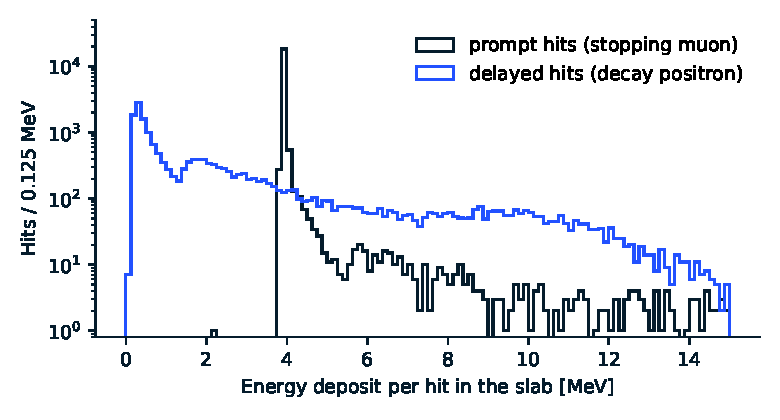
\includegraphics[width=0.78\textwidth]{figures/edep_spectrum.pdf}
\caption{Energy per hit in the slab, from the reference run of \texttt{first\_sim.mac} (log scale). Each muon produces two hits: a \emph{prompt} one as it stops, depositing its full \(\approx\)\SI{4}{MeV} kinetic energy (sharp peak), and a \emph{delayed} one, microseconds later, from its decay positron (broad spectrum). Muons that decay within the \SI{100}{ns} hit-separation window merge both into one prompt hit --- the prompt tail above \SI{4}{MeV}.}
\label{fig:edep}
\end{figure}

\begin{recap}
\begin{itemize}
  \item Macros mix universal Geant4 commands, \musrSim's \code{/musr/command} and \code{/musr/run}, and the \code{/gun} beam.
  \item \code{/musr/command} lines are parsed from the file at start-up; everything else is executed in order afterwards. No \code{/run/initialize}; no \code{/musr/command} in included files.
  \item \code{../musrSim macro.mac idle} gives you a prompt where \code{ls} and \code{help} list the real \code{/gun} and \code{/musr/run} commands.
  \item A complete simulation needs a \code{World}, one sensitive volume, \emph{the physics block}, a beam, and \code{/run/beamOn}.
\end{itemize}
\end{recap}
\nextchap{building real geometry with the \texttt{construct} command}
